% start: template for headers and footer info that need to be adde in each pade that includes a section
\chead{\textit{IT-University of Copenhagen} \rangle  SSEQ-E2013  \rangle \textbf{Group:} 10 Danish Travel card  \rangle \textbf{ID:} 102 \rangle Responsible: All}
\cfoot{\textbf{Hand-in date:} \today \rangle \textbf{Supervisor:} Marco Nardello \rangle \textbf{Version:} 1 \rangle \textbf{Status: } Done \thepage}
\renewcommand{\headrulewidth}{0.1pt}
\renewcommand{\footrulewidth}{0.1pt}
% ends: headers/footers template

\section*{Software Architecture Sketch}

At this part of our project we intend to describe how our system should be organized and designed seen from an overall structure related to our chosen development process, which is the design phase of the waterfall.

\begin{figure}[ht!]
\centering
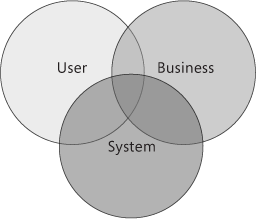
\includegraphics[width=60mm]{graphics/SA_pic_1.png}
%\caption{Chapter 24 page 653}
\label{asw}
\end{figure}

Software architecture can basically be designed either at a small scale or at a larger scale. Architecture at a small scale concentrates at the architecture of individual programs, whereas at a larger scale the whole system is taken to consideration. Since the Rejse Kort system is a larger system, we intend to design the software architecture seen from a larger scale, which will include the most important parts of the system. It worth mentioning there are more factors which are important to take into consideration when designing the architecture. The design should basically take both the user, the system and the business aspects into consideration. These three key points should all have a balanced impact on the output of the design. 

\begin{figure}[ht!]
\centering
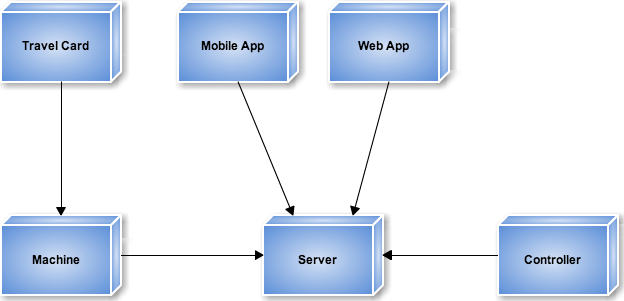
\includegraphics[width=80mm]{graphics/SA_pic_2.png}
%\caption{Chapter 24 page 653}
\label{ano}
\end{figure}


The model clearly illustrates that the components are depending on the server which they are connect to, but the server is not dependent of the other components by it self. All the components being dependent on the server makes the software security quality an important point. It is an important point for the system that the server can function without dependencies. The  design of the server being the main components without dependencies, ables the parts of the system, such as the mobile or web application to work even if the check-in and check-out machines are not functioning.

\begin{figure}[ht!]
\centering
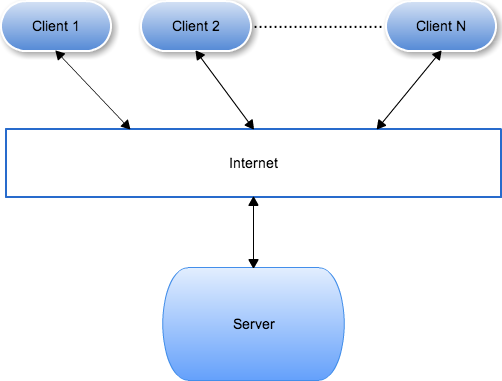
\includegraphics[width=70mm]{graphics/SA_pic_3.png}
%\caption{Chapter 24 page 653}
\label{some}
\end{figure}

We have chosen the well known Client-Server pattern for the system since it lives to the software quality requirements. A general model of the pattern is illustrated below, where N amount of clients are able to “connect” to the server, and the server can likewise send data back to each client depending on their actions and requests.



There are many benefits using the client server pattern, but the main part; High security, Centralized data access and ease of maintenance.These three key point can be directly related to our software qualities. 



A part of the security can be implemented by storing all data on the server, which compared to client machines offers a larger scale of security.
The centralized data access affects the systems reliability, since the clients can be certain that their data, information  etc. is up to date at any time, which is important since they are able to use their Rejsekort, and access their account in different ways. Even though the models we have showed illustrates a single server, multiple servers, that are know to each other, may be used if needed in order to ensure that the client will be unaware and unaffected whenever the system servers are in need of upgrades, repairs etc.



A typical client-server architecture uses multiple server in a larger scale, but in our case a centralized server would be more efficient, and if critically needed other servers may be implemented. The centralized server is need since as we mentioned, all the data need to have a low dependency on other servers in case of failure.